\documentclass[10pt,oneside]{article}
\usepackage[utf8]{inputenc}
\usepackage[T1]{fontenc}
\usepackage{latexsym}
\usepackage[spanish,es-nodecimaldot,es-noshorthands]{babel}
\usepackage{amsfonts}
\usepackage{multicol}
\usepackage{amsmath}
\usepackage{amssymb}
\usepackage{amsthm}
\usepackage[all]{xy}
\usepackage{tikz}
\usepackage[retainorgcmds]{IEEEtrantools}
\usepackage{mathrsfs}
\usepackage{ upgreek }
\usepackage{tcolorbox}
\tcbuselibrary{theorems}
\newtcbtheorem[auto counter, number within = section]{theorems}{Teorema}%
{colframe=gray!50!black,fonttitle=\bfseries}{}
\theoremstyle{definition}
\newtheorem{definition}{Definición}[section]
\usepackage[pdftex]{hyperref}
\addtolength{\hoffset}{-3.5cm}
\addtolength{\textwidth}{7.2cm}
\addtolength{\voffset}{-3cm}
\addtolength{\textheight}{5cm}
\pagestyle{empty}


\title{\textbf{Notas de Modelación Epidémica}}

\author{Lucho Cervantes Jorge Luis}


\begin{document}

\maketitle

\begin{multicols}{2}

\tableofcontents
    \section{Introducción}
    
    \textbf{Epidemiología:} Estudio de una población respecto a su estado de salud. Para esto se definen clases epidemiológicas. La unión de estas clases es resulta en la población. \\ \newline \textbf{Estado de salud:} Según la OMS, estado de bienestar fisiológico, psicológico y social. \\ \newline Se tiene un enfoque en enfermedades causadas por patógenos como virus, bacterias, hongos, priones, etc.
    \textbf{Herramientas matemáticas:}
    
    \begin{enumerate}
        \item \textbf{Estadística}
        \begin{itemize}
            \item Muestreo: cuando el tamaño de muestra es suficientemente grande para hacer buenas predicciones.
            \item Inferencias:
            \begin{itemize}
                \item[*] bayesianas
                \item[*] frecuentistas
            \end{itemize}
        \end{itemize}
        \item \textbf{Azar}: si los datos no son suficientes se puede hacer una aproximación y/o ajuste de datos aleatorios o con una distribución que corresponda con las observaciones. Esto implica cierto grado de incertidumbre (Procesos estocásticos).
        \item \textbf{Aproximaciones de campo medio}: a partir de estas se aplican las ecuaciones diferenciales de la forma:
        $$\frac{dS}{dt}=-\alpha SI+ f(S,I;...)$$
        donde el término $SI$ es no lineal y en general es el que mide cómo interaccionan los individuos de una clase epidemiológica con los de otra. \\ \newline En este caso $S$ es la población susceptible o (saludable) e $I$ es la población infectada. En este tipo de modelos se hace la \textit{hipótesis de la buena mezcla}, i.e. que todos los individuos de $S$ tienen la misma probabilidad de infectarse al contactar un elemento de $I$. Esto no es necesariamente cierto.
        \item \textbf{Redes:} se utilizan para tomar en cuenta las inhomogeneidades que pueden presentar las poblaciones mediante pesos de las conexiones de sus nodos.
        \item \textbf{Herramientas computacionales:}
        \begin{itemize}
            \item Autómatas celulares: abarca la espacialidad y el comportamiento local de los individuos.
            \item Modelos multi agentes: abarca el comportamiento (Problema de la racionalidad acotada).
        \end{itemize}
    \end{enumerate}
    
    \textbf{Enfermedades}
    
    \begin{enumerate}
        \item \textbf{Infecciosas} (patógenos)
        \begin{itemize}
            \item comunicables: se transmiten de persona a persona por contacto directo 
            \item Transmitibles: se transmiten de persona a persona, pero puede ser por vía aérea, por comida infectada, el agua. También enfermedades vectoriales (una persona infecta algún vector, como el mosquito en el dengue, y este a su vez infecta a otra persona) y enfermedades verticales (las que se heredan). 
        \end{itemize} 
        \item \textbf{Sistémicas:} Como la diabetes.
    \end{enumerate} 
    
    Términología que se utiliza respecto al \textbf{estado de la enfermedad}.
    
    \begin{enumerate}
        \item \textbf{Expuesto}: contacto efectivo con un infectado.
        \item \textbf{Infectado}: Si el patógeno se establece en el cuerpo de alguien expuesto. 
        \item \textbf{Infeccioso}: infectado que puede contagiar.
        \item \textbf{Latente}: infectado que no puede contagiar, al menos, por un tiempo (tiempo de latencia).
        \item \textbf{Incubación}: Periodo entre la exposición y la infección.
        \item \textbf{Prevalencia}: Número de infectados en un tiempo específico.
        \item \textbf{Incidencia}: Número de infectados en un intervalo de tiempo.
        \item \textbf{Fatalidad}: Número de muertos por la enfermedad respecto al número de infectados.
        \item \textbf{Mortalidad}: Número de muertos por la enfermedad respecto a la población total.
    \end{enumerate}

    \section{Modelo de Kermack-McKendrick (SIR)}

    Considera enfermedades que se transmiten por contacto, periodo de incubación pequeño, tasa de mortalidad baja, tasa de contagio "alta", duración corta y que genera inmunidad.\\ \newline Se considera la parte de la población susceptible, $S$, la parte infectada, $I$ y la parte removida, $R$, (muertos y recuperados que adquieren inmunidad permanente). Modela, por ejemplo, la varicela y el sarampión de manera aproximada.\\ \newline \textbf{Hipótesis:}

    \begin{itemize}
        \item No hay efectos demográficos debido a la escala de tiempo de la enfermedad (No se consideran los nacimientos ni las muertes naturales).
        \item Población cerrada (No hay efectos de migración).
        \item Población bien mezclada (Toda la población tiene la misma probabilidad de tener un contacto efectivo con un infectado y la misma probabilidad de infectarse).
        \item Inmunidad permanente (Los removidos no infectan).
    \end{itemize}

    La población total, $N$, al tiempo, $t$, es tal que:
    
    \begin{equation}\label{eq:1}
        N(t)=S(t)+I(t)+R(t),
    \end{equation}
    
    donde $cN$ es el contacto efectivo por unidad de tiempo y $S/N$ es la probabilidad de contacto. Entonces, $cN\cdot S/N=cS$ es el contacto efectivo. Definiendo $P$ como la probabilidad de transmisión y $\beta=Pc$ se tiene que la probabilidad de que una persona se infecte es $cS\cdot P=\beta S$. En consecuencia, la tasa de infectados infecciosos es $cSI$. \\ \newline El modelo se representa con el diagrama:
    \begin{center}\vspace{0.3cm}
       \hspace{0.6cm}\xymatrix{*+<0.6cm>[F]{S} \ar[r]^{\beta I} & *+<0.6cm>[F]{I} \ar[r]^{\alpha}&*+<0.6cm>[F]{R}} 
       \vspace{0.3cm}
    \end{center} Donde se expresa que $I$ depende de $\beta S$ y $R$ de la tasa de remoción $\alpha$. El modelo es:

    \begin{equation}\label{eq:2}
         \tcboxmath[colback=white,colframe=gray, title=Modelo de Kermack-McKendrick (SIR)]{\begin{array}{ccl}
            \dot S & = & -\beta SI \\
            \dot I & = & \beta SI - \alpha I\\
            \dot R & = & \alpha I\\
        \end{array}} 
    \end{equation}
    % Para hacer las cajitas de colores solo se requieren  \usepackage{tcolorbox} y \tcbuselibrary{theorems}.
    
    con las condiciones iniciales $S(0)=S_0$, $I(0)=I_0$ Y $R(0)=0$ ($\Rightarrow N_0=R_0+S_0$). En particular 

    \begin{equation}\label{eq:3}
        \dot N=\dot S+\dot I+\dot R\equiv 0; \hspace{0.5cm} N\equiv0. 
    \end{equation}
    
    Considerando:
    
    $$\lim_{t \to\infty }=S_{\infty},$$ $$\lim_{t\to\infty }=I_{\infty},$$ $$\lim_{t\to\infty }=R_{\infty}$$ 
    
    también se tiene que:

    \begin{equation}\label{eq:4}
        N=S_{\infty}+R_{\infty}.
    \end{equation}

    Cuando $I>S$ se dice que hay una epidemia. Para que la población infectada aumente se tiene que: 

    $$\dot I(t)>0\hspace{0.5cm} \forall t$$ $$\Leftrightarrow \hspace{0.5cm}\dot I(t=0)=(\beta S_0-\alpha) I_0>0$$ $$\Leftrightarrow\hspace{0.5cm} \frac{\beta}{\alpha}S_0>1$$

    A $R_0 \equiv\beta S_0/\alpha $ se le conoce como número de reproducción básico y puede pensarse como el número de casos secundarios que produce un único infeccioso en la población susceptible. Si $R_0>1$ hay brote epidémico. Si $R_0\leq1$ no hay brote epidémico. \\ \newline
    Por otro lado, la tercera ecuación de (\ref{eq:2}) es redundante pues $\dot R=\alpha I$ aparece  en la segunda ecuación. Así, el sistema puede resolverse considerando solo las primeras dos ecuaciónes y que 
    
     \begin{equation}\label{eq:5}
         R(t)=\underbrace{N}_{\textnormal{cte.}}-S(t)-I(t).
     \end{equation}

     Comparando $S$ con $R$:

     $$\frac{dS}{dR}=\frac{\frac{dS}{dt}}{\frac{dR}{dt}}=\frac{\dot S}{\dot R}=-\frac{\beta SI}{\alpha I}=-\frac{\beta S}{\alpha}$$ $$\Rightarrow\hspace{0.5cm} S(t)=S_0 e^{\frac{\beta}{\alpha} R}.$$

     Comparando $S$ con $I$:

      $$\frac{dS}{dI}=-\frac{\beta SI}{\beta SI-\alpha I}=-\frac{\beta S}{\beta S-\alpha }$$
      $$\Leftrightarrow\hspace{0.5cm}\int \frac{\alpha-\beta S}{\beta S}dS=\int dI =I$$
      $$\Leftrightarrow\hspace{0.5cm}\int \frac{\alpha-\beta S}{\beta S}dS=\int dI =I$$
      $$\Leftrightarrow\hspace{0.5cm}I=\frac{\alpha}{\beta}\int\frac{dS}{S}-\int dS=\frac{\alpha}{\beta}\ln S-S$$
      $$\Leftrightarrow\hspace{0.5cm} I+S-\frac{\alpha}{\beta}\ln S=\textnormal{cte.} \hspace{0.5cm} \forall t$$

      Para $t=0$
      
      $$\Leftrightarrow\hspace{0.5cm} \underbrace{S_0+I_0}_{=N}-\frac{\alpha}{\beta}\ln S_0= \textnormal{cte.}$$

      Para $t\to \infty$

      $$\Leftrightarrow\hspace{0.5cm} S_{\infty}+\underbrace{I_{\infty}}_{=0}-\frac{\alpha}{\beta}\ln S_{\infty}= \textnormal{cte.}$$

      Entonces:

      $$N-S_{\infty}=\frac{\alpha}{\beta}(\ln S_0-\ln S_{\infty})=\frac{\alpha}{\beta}\ln \frac{S}{S_{\infty}} $$
      $$ \Rightarrow \frac{\beta}{\alpha}=\frac{\ln \frac{S}{S_{\infty}}}{N-S_{\infty}} $$

      La figura \ref{fig:1} Muestran el comportamiento dede las soluciones.
      
      \begin{figure*}
          \centering
          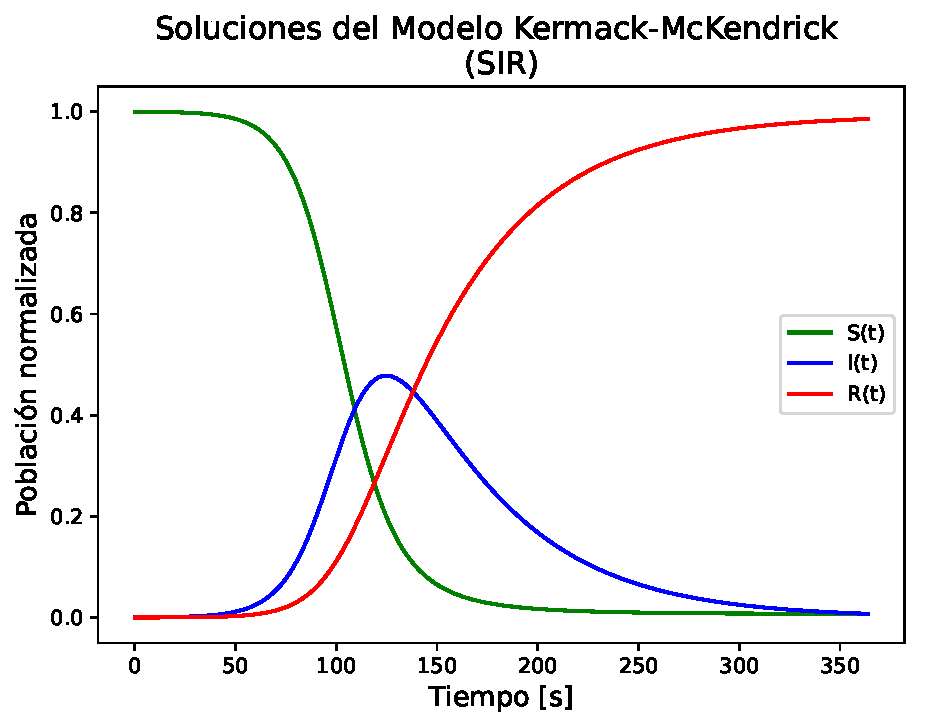
\includegraphics[scale=0.5]{Figuras/f1.pdf}\hspace{0.5cm}
          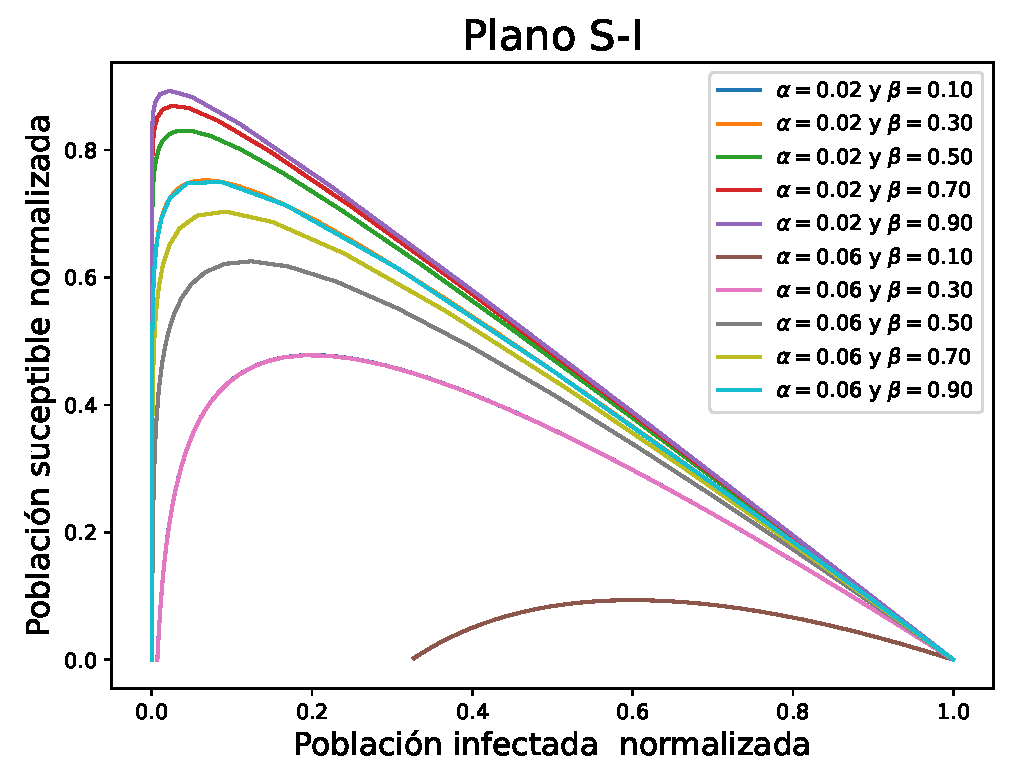
\includegraphics[scale=0.45]{Figuras/f2.pdf}
          \caption{Soluciones del sitema de ecuaciones diferenciales (izquierda). Curvas del plano S-I, variando $\alpha$ y $\beta$ (derecha).}
          \label{fig:1}
      \end{figure*}

    \subsection{estimación del tiempo de recuperación}
    
    Si ya no hay nuevos infecciosos ($\beta SI=0$) entonces 
    
    $$\dot I =-\alpha I$$ $$\Rightarrow \hspace{0.5cm} I(t)=I_0e^{-\alpha t}$$
    $$\Leftrightarrow \hspace{0.5cm} \ln\left(\frac{I(t)}{I_0}\right)=-\alpha t$$
    $$\Leftrightarrow \hspace{0.5cm} \frac{\ln I_0-\ln I(t)}{t}=\alpha $$
    
    En este, caso la probabilidad de ser infeccioso al tiempo $t$ es: 
    
    \begin{equation}\label{eq:6}
        F(t)=1-\frac{I(t)}{I_0}=1-e^{-\alpha t}
    \end{equation}
    
    Entonces la función de densidad de probabilidad es:
    
    \begin{equation}\label{eq:7}
        f(t)=F(t)=\alpha e^{-\alpha t}
    \end{equation}
    
    y la esperanza, que en este caso puede pensarse como el tiempo medio de infección es: 
    
    \begin{equation}\label{eq:8}
        E[X]=\int_{-\infty}^{\infty}tf(t)dt=\int_{-\infty}^{\infty}t\alpha e^{-\alpha t}dt=\frac{1}{\alpha}
    \end{equation}
    
    \subsection{Caso sin remoción}
    
    Suponiendo que los infectados no mueren, pero al curarse son susceptibles de volver a enfermarse (Como una gripe común) se tiene entonces algo del estilo:
    
    \begin{center}
    \hspace{0.4cm}\xymatrix{*+<0.4cm>[F]{S}\ar@/^{8mm}/[r]^{\alpha S} & *+<0.4cm>[F]{I}\ar@/^{8mm}/[l]^{\beta}}    
    \end{center}
    
    En este caso el sistema de ecuaciones es 
    
    \begin{equation}\label{eq:9}
         \tcboxmath[colback=white,colframe=gray, title=Modelo SI]{\begin{array}{ccc}
            \dot S & = & \beta I -\alpha SI \\
            \dot I & = & \alpha SI - \beta I\\            
        \end{array}} 
    \end{equation}
    
    Con
    
    \begin{equation}\label{eq:10}
        N=S(t)+I(t).
    \end{equation}
    
    Tomando $r=\alpha N-\beta$ y $ k=r/\alpha$ se tiene que 
    
    $$\dot I=\alpha SI-\beta I=\alpha (N-I)I-\beta I=\cdots $$ 
    $$\cdots=(\alpha N-\beta)I-\alpha I^2=(\alpha N-\beta)I\left(1-\frac{\alpha}{\alpha N-\beta}I\right)=\cdots$$
    $$\cdots=rI\left(1-\frac{\alpha}{r}I\right)=rI\left(1-\frac{I}{k}\right)$$
    
    i.e. se tiene la ecuación logística
    
    \begin{equation}\label{eq:11}
        \dot I=rI\left(1-\frac{I}{k}\right).
    \end{equation}
    
    Ri $r>0$ entonces $\dot I\leq rI(t) \hspace{0.3cm}\forall t$ por lo que la enfermedad gradualmente desaparece. Si $r>0$ entonces se tiene una epidemia. Considerando que $r=\alpha N-\beta$, estas condiciones se traducen, en términos del número reproductivo básico, en que $R_0=\alpha N/\beta>1$ y  $R_0=\alpha N/\beta<S1$ respectivamente.\\ \newline Para resolver, de la ecuación (\ref{eq:11}) se tiene que:
    
    $$\frac{\frac{dI}{dt}}{I\left(1-\frac{I}{k}\right)}=r$$
    $$\Leftrightarrow \hspace{0.5cm} \int \frac{dI}{I\left(1-\frac{I}{k}\right)}=\int r dt=rt+\zeta_1$$
    $$\Leftrightarrow \hspace{0.5cm} rt+\zeta_1=\int\frac{dI}{I}+\int\frac{dI}{k-I}=\cdots$$ $$\cdots=\ln I- \ln(k-1) + \zeta_2=\ln\left(\frac{I}{k-I}\right)+\zeta_2$$    
    $$\Leftrightarrow \hspace{0.5cm} \frac{I}{k-I}=e^{rt+\zeta_1-\zeta_2}=\underbrace{e^{\zeta_1-\zeta_2}}_{\zeta}e^{rt}$$
    $$\Leftrightarrow \hspace{0.5cm}I=(k-I)\zeta e^{rt}=k\zeta e^{rt}-I\zeta e^{rt}$$  $$\Leftrightarrow \hspace{0.5cm}I(t)=\frac{k \zeta e^{rt}}{\left(1+\zeta e^{rt}\right).}$$
    
   En particular:
   
   $$I_0=I(t=0)=\frac{k\zeta}{1+\zeta}\hspace{0.5cm}\Leftrightarrow\hspace{0.5cm} \zeta=\frac{I_0}{k-I_0}$$
   
   \subsection{Caso sin remoción pero con tratamiento de recuperación}

   Inicialmente $\beta$ era la recuperación. Considerando una recuperación de la forma $\overline{\beta}=\beta/(1+I)$, se tiene entonces el sistema:

   \begin{equation}\label{eq:12}
         \tcboxmath[colback=white,colframe=gray, title=Modelo SI]{\begin{array}{ccc}
            \dot S & = & \frac{\beta I}{1+I} I -\alpha SI \\
            \dot I & = & \alpha SI - \frac{\beta I}{1+I}\\            
        \end{array}} 
    \end{equation}

    donde, por la ecuación (\ref{eq:10}) se tiene que 

    \begin{equation}\label{eq:13}
        \dot I=\alpha I(N-I)-\frac{\beta I}{1+I}
    \end{equation}

    cuyas soluciones estacionaras ($\dot I\equiv0$) se obtienen de 

    $$\alpha I(N-I)=\frac{\beta I}{1+I}\hspace{0.5cm}\Leftrightarrow\hspace{0.5cm} (N-I)(1+I)=\frac{\beta I}{\alpha I}=\frac{\beta }{\alpha }$$

    que es una parábola.

    \section{Modelo SIR con demografía.}
    En este caso, se considera que la enfermedad permanece en la población el suficiente tiempo para apreciar los efectos de las tasas naturales de natalidad, $\Lambda$, y de mortalidad, $\mu$. I.e. se tiene un caso de la forma:

    \begin{center}
       \vspace{0.5cm}
       \hspace{0.6cm}\xymatrix{\ar[r]^{\Lambda}&*+<0.6cm>[F]{S} \ar[r]^{\alpha S}+\ar[d]^{\mu} & *+<0.6cm>[F]{I} \ar[r]^{\beta} +\ar[d]^{\mu}&*+<0.6cm>[F]{R} \ar[d]^{\mu}\\&&&}
       \vspace{0.5cm}
    \end{center}

    Con el sistema de ecuaciones diferenciales:

    \begin{equation}\label{eq:14}
         \tcboxmath[colback=white,colframe=gray, title=Modelo SIR con demografía]{\begin{array}{ccl}
            \dot S & = & \Lambda -\alpha SI -\mu S \\
            \dot I & = & \alpha SI - \beta I - \mu I \\
            \dot R & = & \beta I -\mu R\\
        \end{array}} 
    \end{equation}

    En este caso la ecuación (\ref{eq:1}) también es válida sin embargo, se tiene que 

    \begin{equation}\label{eq:15}
        \dot N= \dot I+ \dot S+ \dot R=\Lambda-\mu(\underbrace{S+I+R}_{=N})
    \end{equation}

    Considerando la solución estacionaria ($\dot N\equiv0$), se tiene que $N=\Lambda/\mu$. En particular, cuando $t\to \infty$ debe ocurrir que $N_{\infty}=\Lambda/\mu$\\\newline Como $R$ se puede escribir en términos de $N,I$ y $S$ entonces es redundante (en términos de álgebra lineal, se puede ver como combinación lineal de las otras soluciones). De manera que podemos considerar solo las dos primeras ecuaciones del sistema. Más aún lo consideraremos adimensionalizado. Tomando $\tau=(\alpha+\mu)t$ se tiene que
    
    $$\frac{dS}{d\tau}=\frac{1}{\beta+\mu}\frac{dS}{dt}$$
    $$\frac{dI}{d\tau}=\frac{1}{\beta+\mu}\frac{dI}{dt}$$
    
    y tomando $\displaystyle{x=\frac{\mu}{\Lambda}S}$, $\displaystyle{y=\frac{\mu}{\Lambda} I}$, $\displaystyle{\rho=\frac{\mu}{\beta+\mu}}$ y $\displaystyle{R_0=\frac{\Lambda \alpha}{\mu(\beta+\mu)}}$ se tiene el sistema:

    \begin{equation}\label{eq:16}
    \begin{array}{cl}
         \displaystyle{\frac{dx}{d\tau}}=& \rho(1-x)-R_0xy \\ 
         \displaystyle{\frac{dy}{d\tau}}=& (R_0x-1)y 
    \end{array}  
    \end{equation}

    Encontrando los puntos fijos:

    $$\rho(1-x)-R_0xy=0$$
    $$(R_0x-1)y=0$$

    En el caso en que no hay infectados ($y=0$) necesariamente $x=1$. Por lo que $E_0=(1,0)$ es el equilibrio libre de enfermedad. Si $y\neq 0$ entonces, de la primera ecuación: 

    $$\rho(1-x)=R_0xy\hspace{0.5cm}\Leftrightarrow\hspace{0.5cm}\frac{\rho(1-x)}{R_0x}=y$$

    y de la segunda ecuación, $x=\displaystyle{\frac{1}{R_0}}$, con lo cual:

    $$y=\frac{\rho\left(1-\frac{1}{R_0}\right)}{R_0\frac{1}{R_0}}=\rho\left(1-\frac{1}{R_0}\right)$$

    Con lo que $\displaystyle{E=\left(\frac{1}{R_0}, \rho\left(1-\frac{1}{R_0}\right)\right)}$ es un punto de equilibrio. Si $R_0<1\hspace{0.5cm}\Rightarrow\hspace{0.5cm}\left(1-\frac{1}{R_0}\right)<0$ de manera que el punto no es fe asible o de interés biológico. Si $R_0=1$ entonces $E$ se encuentra sobre el eje de los susceptibles, con lo cual no hay infecciosos, por lo que no es un caso interesante. Si $R_0>1$ entonces $E \in (\mathbb{R_+}\times\mathbb{R_+})$ y si es de interés biológico. En este caso se conoce como equilibrio endémico.\\ \newline
    Considerando el cambio de la población infeciosa repecto al cambio de la población susceptible:

    $$\frac{dy}{dx}=\frac{R_0x-1}{(1-x)-R_0xy}=\frac{f(x,y)}{g(x,y)}$$

    Se tienen las cero-clinas $y=0, \displaystyle{y=\frac{\rho(1-x)}{R_0x}}$ y $\displaystyle{x=\frac{1}{R_0}}$. \\\newline

    \subsection{Linealización y un análisis local de los puntos de equilibrio.} Para la  linealizar el sistema (\ref{eq:16}) se toman derivadas parciales respeto a $x $ y $y$. I.e. la matríz jacobiana es tal que 

    $$J_{(X,Y)}=\left(\begin{array}{cc}
       -\rho-R_0y  & -R_0x \\
       R_0y  & R_0x-1
    \end{array}\right)$$

    De manera que en $E_0=(1,0):$
    
    $$J_{E_0}=\left(\begin{array}{cc}
       -\rho  & -R_0 \\
       0 & R_0-1
    \end{array}\right)$$

    Así, el polinomio característico es tal que

    $$p(\lambda)=\det (J_{E_0}-\lambda I)=\det \left(\begin{array}{cc}
       -\rho-\lambda  & -R_0 \\
       0 & R_0-1-\lambda
    \end{array}\right)=\cdots$$
    $$\cdots=(-\rho-\lambda)(R_0-1-\lambda)$$

    con los valores própios $\lambda_1=-\rho<0$ y $\lambda_2=R_0-1$. Si $R_0<1$ entonces $E_0$ es estable asintóticamente. Si $R_0>1$ entonces  $E_0$ es punto silla. \newline En el caso del equilibrio endémico ($R_0<1$):
    
    $$J_{E}=\left(\begin{array}{cc}
       -\rho-R_0y  & -R_0x \\
       R_0Y & 0
    \end{array}\right)\hspace{0.5cm}$$

    con $tra(J_{E})<0$ y $\det(J_E)=R_0^2xy>0$. Esto implíca que $E$ es localmente asintóticamente estable. Haciendo un análisis similar al de $E_0$ se concluye que los valores propios del polinomio característico en este caso son:

    $$\lambda_{1,2}=\rho R_0 \pm \frac{\sqrt{D}}{2}\hspace{0.5cm}  D=(\rho R_0)^2-4\rho(R_0-1)$$

    En este caso, $D>0$ implica que $E$ es un nodo y $D<0$ que es una fuente.

    \subsection{Estabilidad Global}

    \begin{theorems}{}{t1}
        Si $R_0<1$ entonces $E_0$ es globalmente asintóticamente estable.
    \end{theorems}

    \textbf{Demostración:} Como en $x(0)>1\Rightarrow\displaystyle{\frac{dx(\tau)}{d \tau}<0}$ Entonces $x(\tau)$ es decreciente si $x>1$. Suponiendo que $\exists\hspace{0.3cm} \tau_0>0$ tal que $x(\tau_0)=1$ entonces $\left.\frac{dx(\tau)}{d \tau}\right\vert _{\tau_0}<1$ y $x(\tau)\leq1 \hspace{0.3cm}\forall \tau\geq \tau_0$, Si $x(0)\leq$ se toma $\tau_0=0$ entonces $\frac{dy(\tau)}{d\tau}=(R_0x-1)y(\tau)$ es tal que para $\tau\geq\tau_0$ se tienen que $\frac{dy(\tau)}{d\tau}\leq(R_0-1)y(\tau)$. Integrando esto se tiene:

    $$y(\tau)=y(\tau_0)e^{(R_0-1)(\tau-\tau_0)}.$$ 

    Como $R_0<1$ entonces $\displaystyle{\lim_{\tau \to \infty}}y(\tau)=0$.\\ \newline Por otro lado, sabemos que $\lim_{\tau\to \infty}^{Sup} x\leq1$. Haciendo un tratamiento análogo al de $y(\tau)$ se llega a que:
    
    \begin{equation}\label{eq:17}
    x(\tau)\leq e^{-\rho\tau}x(0)+\rho\int_0^{\tau}e^{-\rho(\tau-S)dS}.
    \end{equation}

    Como $\displaystyle{\lim_{\tau \to \infty}}y(\tau)=0$ entonces $\forall\varepsilon>0\hspace{0.3cm}\exists$ $\tau_0>0$ t.q. $y\leq\varepsilon$ para $\tau>\tau_0$ Tomando esos valores de $\tau$:

    $$\frac{dx\tau}{d\tau}\geq \rho(1-x)-\varepsilon R_0x(\tau)$$

    que aunado a la desigualdad (\ref{eq:17})

    $$x(\tau)\geq e^{-(\rho+\varepsilon R_0)\tau}x(0)+\rho\int_0^{\tau}e^{-(\rho+\varepsilon R_0) (\tau-S)}dS$$

    con lo cual $\lim_{\tau\to\infty}^{Inf}x\geq\frac{\rho}{\rho+\varepsilon R_0}$ $\forall\varepsilon>0$, es decir  $\lim_{\tau\to\infty}^{Inf}x\geq1$. Por tanto $\lim_{\tau\to\infty}x=1$. Con lo cual $E_0$ es un punto globalmente asintóticamente estable.

    \subsubsection{Paréntesis (resultados necesarios)}

    Sea $u(t)=(x(t), y(t))$ una curva parametrizada con la condición inicial $U_0=(x(0),y(0))$.   

    \begin{definition}[Conjunto $\omega$- límite de $u_0$]
        Es el conjunto de todos los puntos $a\in \mathbb{R}^2$ para los cuales $\exists$  $(t_j)$ t.q. $u(t_j)\to a$ cuando $t_j\to \infty$. Se denota por $\omega(u_0)$.
    \end{definition}

    \begin{definition}[Órbita  homoclínica]
        Es la trayectoría del flujo de un sistema dinámico que une a un punto silla con consigo mismo.
    \end{definition}
    
    \begin{definition}[Órbita  heteroclínica]
        Curva en el plano fase que une dos puntos de equilibrio diferentes.
    \end{definition}
    
    \begin{definition}[Separatríz]
        Curva en el plano fase que toca un equilibrio hiperbólico o conecta una variedad estable con una inestable de un par de puntos de equilibrio.
    \end{definition}
    
    \begin{definition}[Ciclo separatriz]
        Unión finita de puntos de quilibrio $P_j$ con $j=1,...,m$ y separatrices $\Gamma_j$ t.q. el flujo sobre $\Gamma_j$ va de $P_j$ a $P_{j+1}$ y $P_{m+1}=P_1$ .
    \end{definition}

    \begin{definition}[Ciclo separatríz compuesto]
        Unión finita de ciclos separatrices compatibles en orientación ~\cite{Mod:epid}.
    \end{definition}

    \begin{theorems}{Teorema de Poincaré-Bendixson}{t2}
        Sea $X\subseteq\mathbb{R}^2$ un abierto que contiene una cantidad finita de puntos de equilibrio, y sea $u(t)$ una solución en $X$ acotada y no negativa t.q. $\omega(u_0)\subseteq X$. Entonces, $\omega(u_0)$ es un punto de equilibrio $\lor$ $\omega(u_0)$ es una órbita periódica, $\lor$ $\omega(u_0)$ es un ciclo separatríz compuesto.   
    \end{theorems}

    La prueba de este teorema corresponde a un curso de ecuaciones difrenciales, pero puede encontrarse en ~\cite{PBteorema}.

    \begin{theorems}{Criterio de Dulac-Bendixson}{t3}
        Sea $Z\subseteq X $ un abierto simplemente conexo. Sean $\dot x=f$ y $\dot y=g$ de clase $\mathcal{C}^{1}$ en $Z$. Suponiendo que $\exists\hspace{0.3cm}D: Z\longrightarrow\mathbb{R}$ clase $\mathcal{C}^{1}$ en $Z$ t.q. $\partial_x(Df)+\partial_y(Dg)\leq 0$ (ó $\geq0$) en un conjunto de medida cero en $Z$. Entonces, $Z$ no tiene órbitas periódicas ni ciclos separatrices compuestos. \\ \newline A $D$ se le conoce como función de Dulac. 
    \end{theorems}

    La prueba de este teorema puede encontrarse en ~\cite{dulacben}, \\ \newline Considerando el sistema reducido y adimensionalizado (\ref{eq:16}) Se tienen los siguientes resultados:

    \begin{theorems}{}{t4}
        Si $R_0$>1, entonces el sistema (\ref{eq:16}) no tiene órbitas periódicas ni ciclos separatrices.  
    \end{theorems}

    \textbf{Demostración:} Considerando $f(x,y)=\dot x$ y $g(x,y)=\dot y$ y $Z=(0,\infty)\times(0,\infty)$, y $D\equiv 1$ se tiene que

    $$\partial_x(Df)+\partial_x(Dg)=\partial_xf+\partial_xg=-\rho-R_0y+R_0x-1$$

    Esto nos sugiere proponer $D(x,y)=\displaystyle{\frac{1}{y}}$ que es $\mathcal{C}^{1}$ en $(0,\infty)\times(0,\infty)$. Así

    $$\partial_x(Df)+\partial_x(Dg)=-\frac{\rho}{y}-R_0<0$$

    De modo que, por el criterio de Dulac-Bendixson (\ref{eq:16}) se concluye lo deseado.

    \begin{theorems}{}{t5}
        Si $R_0$>1 y $I(0)$, entonces el punto de equilibrio $E$, del sistema (\ref{eq:16}), es globalmente estable.  
    \end{theorems}

    \textbf{Demostración:} Tomando $\hat{\rho}=\min\{\rho,1\}$ entonces
    
    $$\dot x + \dot y\leq \rho-\hat{\rho}(x+y)$$
    $$(x+y)\leq\kappa e^{-\hat{\rho}}+\frac{\rho}{\hat{\rho}}\left(1-e^{-\hat{\rho t}}\right)$$

    con $\kappa$ la condición inicial de $x+y$ y $\displaystyle{\lim_{t\to \infty} Sup \{x+y\}\leq \frac{\rho}{\hat{\rho}}}$. Esto implica que las suluciones de (\ref{eq:16}) son acotadas. Ahora, como en $(0,\infty)\times(0,\infty)$ es 

    \section{Ecología de poblaciones que interactúan}

    \subsection{Modelo de Lotka-Volterra}

    Modelo que simula como se relacionan dos poblaciones, una de presas, $x_1$, y otra de depredadores $x_2$.

     \begin{equation}\label{eq:18}
         \tcboxmath[colback=white,colframe=gray, title=Modelo Ross-MacDonald]{\begin{array}{ccc}
            \dot x_1 =& \alpha x_1-\beta x_1 x_2   \\
            \dot x_2 =&  \delta x_1x_2-\gamma x_2           
        \end{array}} 
    \end{equation}

    En particular, su matriz jacobiana (obtenida al linealizar), es:

    $$J=\left(\begin{array}{cc}
       \alpha-\beta x_2  & -\beta x_1 \\
        \delta x_2 & \delta x _1-\sigma
    \end{array}\right)$$

    Este modelo se puede generalizar de la siguiente forma:
    
     \begin{equation}\label{eq:19}
         \tcboxmath[colback=white,colframe=gray, title=Modelo Ross-MacDonald]{\begin{array}{ccc}
            \dot x_1 =&\displaystyle{ r_1x_1\left(1-\frac{x_1}{k_1}\right) + a_{12}x_1x_2 }\\ \\
            \dot x_2 =&  \underbrace{r_2x_2\left(1-\frac{x_2}{k_2}\right)}_{\textnormal{comp logístico}} + a_{21}x_1x_2          
        \end{array}} 
    \end{equation}

    Desarrollando el sistema (\ref{eq:19}) y  definiendo $a_{11}=\frac{r_1}{k_1}$ y $a_{22}=\frac{r_2}{k_2}$ se puede reescribir de forma matricial como

    \begin{equation}\label{eq:20}
        \frac{d\overline{X}}{dt} = \overline{R}^t\hspace{0.1cm}\overline{X}+\overline{X}^{T}M\overline{X} 
    \end{equation}

    donde $\overline{X}^t=(x_1,x_2)$, $\overline{R}^t=(r_1,r_2 )$ y $M=\left(\begin{array}{cc}
       a_{11} & a_{12} \\
       a_{21} & a_{22}
    \end{array}\right)$.
    
    A $M$ se le conoce como matriz ecológica; a sus elementos $a_ii$ como los términos de interacción intraespecífica y a sus elementos $a_{ij}$ con $i\neq j$ cmo sus términos de interacción interespecífica. La ventaja de la ecuación (\ref{eq:20}) es que generaliza el modelo de Lotka-Volterra a la interacción de más de dos especies. \\\newline  En general, si 

    \begin{equation}\label{eq:21}
    \begin{array}{c}
        \dot x_1 = f_1(t_1, x_1,...x_n)  \\
        \dot x_2 = f_2(t_1, x_1,...x_n)  \\
             \vdots  \\
        \dot x_3 = f_3(t_1, x_1,...x_n) 
    \end{array} \hspace{0.1cm}\equiv\hspace{0.1cm} \frac{d \overline{X}}{dt}=F(t,\overline{X})= (f_1,...,f_n)
    \end{equation}


    Para conocer el comportamiento su comportamiento linealizado se tiene que obtener la matriz jacobiana de $F$. En el contexto ecológico, si el sistema anterior representa la interacción de $n$ especies que interactúan entre si entonces se tendrá que $M=DF_p=(\frac{\partial f_i}{\partial x_j})_{ij}$ es la jacobiana del sistema. En tal caso se tiene la siguiente\\ \newline\textbf{Definición:} El sistema (\ref{eq:21}) es cooperativo si $0\leq\frac{\partial f_i}{\partial x_j} \forall i\neq j$  y es competitivo si $\frac{\partial f_i}{\partial x_j}\leq 0 \forall i\neq j$.\\ \newline\textbf{Definición:} Un sistema que es cooperativo o competitivo es llamado monótono. Son requeridos los siguientes resultados

    \begin{theorems}{}{}
       Toda solución acotada de un sistema monótono en $\mathbb{R}^2$ tiende a un punto en equilibrio
\end{theorems}
    
    \begin{theorems}{}{}
       Sea un sistema monótono y $D\subseteq\mathbb{R}^3$ convexo y compacto que no contiene puntos de equilibrio, entonces, toda solución que existe y permanece en $D$ para $0\leq t$ o es periódica, o tiende en espiral a una solución periódica cuando $0\leq t$.
    \end{theorems}

    Los sistemas monótonos se pueden generalizar tomando los conjuntos $$k_m=\{\overline{X}\in \mathbb{R}^n|(-1)^{m_i}x_i\geq 0, 1\leq i\leq n\}$$ con $m=(m_1,...,m_n);$ $m_i\in \{0,1\}$ Los cuales son conjuntos que generan el orden parcial $\leq_m$ dado por : $$ \overline{X}\leq_m\overline{Y}\Leftrightarrow \overline{Y}-\overline{X}\in K_m$$

    \textbf{Definición:} El sistema \ref{eq:21} es $k_m$ cooperativo si $\exists$ si existe una matriz diagonal $H=diag\left((-1)^{m_i}\right)$ con $m_i\in \{0,1\}$ e $i \in \{1,...,n\}$ tal que todos los elemnetos fuera de la diagonal de $H^{-1}DF_{\overline{X}}H$ son no negativos i.e. $$(-1)^{m_1+m_j}\frac{\partial f_i}{\partial x_i}(\overline{X})\geq0$$ y es $k_m$ competitivo si $$(-1)^{m_1+m_j}\frac{\partial f_i}{\partial x_i}(\overline{X})\leq0$$ En particular, un sistema $k_m$ monótono preserva el orden parcial $\leq_m$

    
    \subsection{Transmisión vectorial (Modelo Ross-MacDonald)}

    Sirve para modelar enfermedades como la malaria, la cual es trasmitida por el mosquito anopheles. A su vez, un mosquito sano se infecta cuando pica a un humano infectado. Si $N$ es la población de humanos y $V$ es la de mosquitos, ambas constantes (se descarta la demografía) y $X$, $Y$ son las poblaciones infecciosas de humanos y mosquitos respectivamente, entonces, la población susceptible de humanos es $N-X$ y la de mosquitos es $V-Y$. \\ \newline Como no se sabe cuando alguien es picado por un mosquito infeccioso, el parámetro que indica la velocidad de transmisión es el número de picaduras promedio que un mosquito hace por día, $b$. Así, las picaduras por persona en un día es $\frac{bV}{N}$, $\Rightarrow$ las picaduras que recibe por mosquitos infecciosos es $\frac{bV}{N}\frac{Y(t)}{V}=\frac{bY(t)}{N}$, $\Rightarrow$ las personas susceptibles picadas por mosquitos infecciosos es $\frac{bY(t)}{N}(N-X(t))$. Si $\alpha$ es la fracción de picaduras de mosquitos infecciosos que son efectivas (efectividad de transmisión) entonces $\frac{\alpha bY(t)}{N}(N-X(t))$ son las personas susceptibles que se infectan.\\ \newline En el caso de los mosquitos, la fracción del promedio de picaduras que son a personas infectadas, por mosquito es $\frac{bX(t)}{N}$ $\Rightarrow$ la población de mosquitos que pica a alguien infectado es $\frac{bX(t)}{N}(V-Y(t))$ $\Rightarrow$ la población de mosquitos que se infecta es $\frac{\delta bX(t)}{N}(V-Y(t))$. \\ \newline
    Considerando que los humanos se recuperan (vuelven a ser susceptibles) a una tasa $\mu$ proporcional al número de infectados. En el caso de los mosquitos, se supone que estos viven poco, de manera que si uno es infectado, este morirá infectado, por lo que solo interesa la tasa de mortalidad $\nu$ en general. \\ \newline Definiendo $m=\frac{V}{N}$ y normalizando el sistema (tomando $x=\frac{X}{N}$ y $y=\frac{Y}{v}$), el sistema de ecuaciones diferenciales está dado por:

    \begin{equation}\label{eq:22}
         \tcboxmath[colback=white,colframe=gray, title=Modelo Ross-MacDonald]{\begin{array}{ccc}
            \dot x =& \alpha bm y(1-x)-\mu x  \\
            \dot y =&  \delta b x(1-y)-\nu y           
        \end{array}} 
    \end{equation}

    Pensándolo como un sistema de la forma $\frac{d\overline{X}}{dt}=F(x,y,t)$ se tiene que la matriz jacobiana del sistema es:
    
    $$J=DF_{\overline{x}}=\left(\begin{array}{cc}
        -\alpha bmy-\mu & \alpha bm(1-x) \\
         \delta b(1-y)  & -\delta bx-\nu
    \end{array}\right)$$

    Por otro lado, sus puntos de equilibrio:

    $$\begin{array}{rl}
         0=&\alpha bm y(1-x)-\mu x \\
         0=&\delta b x(1-y)-\nu y
    \end{array} \Leftrightarrow \begin{array}{rl}
        x=& \displaystyle{\frac{\nu y}{\delta b(1-y)}} \\
        y=& \displaystyle{\frac{\mu x}{\alpha bm(1-x)}}
    \end{array}$$

    sustituyendo el valor de $y$ en la expresión de $x$ se tiene que 
    
    $$x=\frac{\mu\nu x}{\delta b^2\alpha m(1-x)-\mu x}$$
    
    Nos interesan los equilibrios no triviales, por lo que suponemos $x_p,y_p\neq0$. Así, se resuelve para $x_p$ como 
    
    $$x_p=\frac{\alpha b^2\delta m -\nu\mu}{\delta b(\alpha bm+\mu)}$$
    
    con lo cual $y_p=\displaystyle{\frac{\mu x_p}{\alpha bm(1-x_p)}}$.\\ \newline Ahora, $E_p=(x_p,y_p)\subseteq D \Leftrightarrow 0< x_p,y_p< 1$. En efecto, 

    $$x_p=\underbrace{\frac{\alpha b^2\delta m}{\delta b(\alpha bm+\mu)}}_{=\frac{\alpha bm}{\alpha bm+\mu}<1}-\underbrace{\frac{\nu\mu}{\delta b(\alpha bm+\mu)}}_{>0}<1$$

    por otro lado:

    $$x_p=\frac{\alpha b m}{\alpha bm+\mu}-\frac{\nu\mu}{\delta b(\alpha bm+\mu)}<\frac{\alpha b m}{\alpha bm+\mu}$$

    $$\Leftrightarrow\hspace{0.3cm} (\alpha bm+\mu)x_p<\alpha bm$$
    $$\Leftrightarrow\hspace{0.3cm} y_p=\frac{\mu x_p}{\alpha bm(1-x_p)}<1$$

    Por lo que se satisfacen las condiciones del teorema 4.2. En particular, consideraremos $R_0^2=S_0=\frac{\alpha b^2\delta m}{\nu\mu}$. \\\newline
    Para el análisis local:

    $$J_{E_p}=\left(\begin{array}{cc}
        -\mu & \alpha bm \\
        \delta b & -\nu
    \end{array}\right); \hspace{0.5cm} p(\lambda)=\lambda^2+(\mu+\nu)\lambda+(\nu\mu-\alpha\delta b^2m)$$

    Para $S_0<1$ las raíces del polinomio característico, $\lambda_1, \lambda_2$ tienen parte real negativa y las soluciones tienden (por el teorema 4.2) a $E_0=(0,0)$. Para $S_0>1$ $Re(\lambda_i)>0$ para alguna $i$, por lo que $E_p$ es un punto silla y las soluciones tienden a $E_p$.

    Si $R_0=1$ entonces se tiene la población crítica de mosquitos $$V_c=\frac{\nu\mu N}{\alpha\delta b^2}$$ La cual determina si se da un brote infeccioso. 

    
    \subsection{Modelo SEIR}

      \begin{center}
       \vspace{0.5cm}
       \hspace{0.6cm}\xymatrix{\ar[r]^{\Lambda}&*+<0.6cm>[F]{S} \ar[r]^{\alpha \frac{SI}{N}}+\ar[d]^{\mu} & *+<0.6cm>[F]{E} \ar[r]^{\sigma } +\ar[d]^{\mu}&*+<0.6cm>[F]{I} \ar[r]^{\beta } +\ar[d]^{\mu}&*+<0.6cm>[F]{R} \ar[d]^{\mu}\\&&&&}
       \vspace{0.5cm}
    \end{center}

    con $$N=S+I+E+R \hspace{0.2cm}\Leftrightarrow\hspace{0.2cm} R=N-S-I-E$$
    Cosiderando una población constante ($\mu=\nu$), al normalizar ($s=\frac{S}{N}$, $i=\frac{I}{N}$, $e=\frac{E}{N}$ y $r=\frac{R}{N}$ ) se tiene el sistema de ecuaciones:

    \begin{equation}\label{eq:23}
         \tcboxmath[colback=white,colframe=gray, title=Modelo Ross-MacDonald]{\begin{array}{ccc}
            \dot s =& \mu -\alpha si -\mu s  \\
            \dot e =& \alpha si -\sigma e -\mu e \\
            \dot i =& \sigma e -\beta i  -\mu i \\
            \dot r =& \beta i  -\mu r \\        
        \end{array}} 
    \end{equation}

    De manera análoga a la ecuación (\ref{eq:15}) se tiene que $\dot N=\Lambda-\mu N$, pero al ser $\Lambda=\mu$, se tiene que: $$\dot N=\mu(1-N).$$ Como $r=1-s-i-e$, la ecuacion correspondiente es redundante por lo que nos quedamos con el sistema sei. Este puede reescribirse como:

    $$\begin{array}{rl}
         \dot s=& -\alpha si-\mu(1-s)  \\
         \dot e =& \alpha si -(\mu+\sigma)e  \\
         \dot i=&\sigma e -(\mu+\beta)i   
    \end{array}$$

    Con el dominio $D_1=\{(s,e,i) \in \mathbb{R}^3_+\hspace{0.1cm}|\hspace{0.1cm}s+e+i\leq1\}$. En particular en $\partial D_1=\{(s,e,i) \in \mathbb{R}^3_+\hspace{0.1cm}|\hspace{0.1cm}s+e+i=1\}$ el campo vectorial apunta hacia el interior de $D_1$. Esto implica, por el principio de invariancia de Lasalle, que las soluciones permanecen dentro de $D_1.$\\ \newline Por otro lado, la jacobiana del sistema es:

    $$J_{(s,e,i)}\left(\begin{array}{ccc}
        \mu-\alpha i &0 &-\alpha s \\
        \alpha i & -(\mu+\sigma)&\alpha s \\
         0&\sigma &-(\mu+\beta)
    \end{array}\right)$$

    Proponiendo $H=\displaystyle{\left(\begin{array}{ccc}
         1& 0 &0\\
         0& -1 &0\\
         0& 0 & 1
    \end{array}\right)}$
    
    Se tiene el cono $k_m=\{(s,e,i)|s\geq, e\leq, i\geq \}$ por lo que el sistema es $k_m$ cooperativo. \\\newline De acuerdo con los teoremas 4.1 y 4.2 las soluciones del sistema tienden a puntos de equilibrio o a soluciones periódicas. \\ Para encontrar los puntos de equilibrio se toma 

    $$\begin{array}{rl}
        \mu -\mu s-\alpha si &=0  \\
         \alpha si -(\mu+\sigma)e&=0  \\
        \sigma e -(\mu+\beta)i &=0 
    \end{array}$$

    En el equilibrio libre de enfermedad ($i\equiv 0$, $e\equiv0$): 

    $$\mu=\mu s \Rightarrow s\equiv 1$$ Por lo que se tiene el punto de equilibrio $E_0=(1,0,0)$. \\ \newline Suponiendo que $s,e,i \neq0$ y considerando que en este caso $R_0=\displaystyle{\frac{\alpha\sigma}{(\sigma+\mu)(\beta+\mu)}}$ Despues de toda el álgebra se obtiene el punto de equilibrio: 
    
    $$E_1=(s^
    *, e^{*}, i^*)=\left(\frac{1}{R_0},\frac{(\beta+\mu)i^*}{(\sigma+\mu)(\beta*\mu)},\frac{\mu\sigma(R_0-1)}{(\sigma+\mu)(\beta+\mu)R_0}\right)$$

    El cual es de interés biológico solo cuando $R_0>1$. Para la estabilidad de $E_0$ se tiene la matriz jacobianas:

    $$J_{E_0}=\left(\begin{array}{ccc}
       -\mu  & 0 & -\alpha\\
        0 & -(\sigma+\mu) &\alpha \\
        0 & \sigma & -(\beta+\mu)
    \end{array}\right)$$
    
    y su correspondiente polinomio característico: 
    $$p(\lambda)=\lambda^2+(2\mu+\sigma+\beta)\lambda+(\sigma+\mu)(\beta+\mu)-\alpha\sigma$$

    El cual tiene ambas raíces negativas si y solo si $R_0<1$, de este modo $E_0$ es estable. \\\newline En el caso de $E_1$, se tiene el polinomio característico:

    $$p(\lambda)=\lambda^3+a_1\lambda^2+a_2\lambda+a_3\hspace{0.2cm} \textnormal{con:}$$

    $$\begin{array}{cc}
         a_1=&2\mu+\sigma+\beta  \\
         a_2=&\mu(a_1)R_0  \\
         a_3=&\sigma\mu\alpha\displaystyle{\left(\frac{R_0-1}{R_0}\right)} 
    \end{array}$$

    donde se satisface que $a_i>0$ $\forall i$ y $a_1a_2>a_3$. Así, por el criterio de Routh Hurwitz, $E_1$ es localmente estable (nuevamente reiterando que $R_0>1$).
    
    

    
    
    
\end{multicols}
   

    
\bibliographystyle{ieeetr}
\addcontentsline{toc}{chapter}{Bibliografía}
\bibliography{biblio.bib}



\end{document}
